\documentclass[11pt,a4paper]{article}

\usepackage[utf8]{inputenc}
\usepackage[T1]{fontenc}
\usepackage[portuguese]{babel}
\usepackage{amsmath}
\usepackage{amsfonts}
\usepackage{graphicx}
\usepackage{geometry}
\usepackage{xcolor}
\usepackage{booktabs}
\usepackage{hyperref}
\usepackage{listings}

\geometry{left=2.5cm, right=2.5cm, top=3cm, bottom=3cm}

% --- Configuração para exibição de código Python ---
\definecolor{codegreen}{rgb}{0,0.6,0}
\definecolor{codegray}{rgb}{0.5,0.5,0.5}
\definecolor{codepurple}{rgb}{0.58,0,0.82}
\definecolor{backcolour}{rgb}{0.95,0.95,0.92}

\lstdefinestyle{mystyle}{
    backgroundcolor=\color{backcolour},
    commentstyle=\color{codegreen}\bfseries,
    keywordstyle=\color{blue},
    numberstyle=\tiny\color{codegray},
    stringstyle=\color{codepurple},
    basicstyle=\ttfamily\footnotesize,
    breakatwhitespace=false,
    breaklines=true,
    captionpos=b,
    keepspaces=true,
    numbers=left,
    numbersep=5pt,
    showspaces=false,
    showstringspaces=false,
    showtabs=false,
    tabsize=4,
    % acentos dentro do código (o listings não aceita UTF-8 multibyte)
    literate={á}{{\'a}}1 {à}{{\`a}}1 {â}{{\^a}}1 {ã}{{\~a}}1 {é}{{\'e}}1 {ê}{{\^e}}1
             {í}{{\'i}}1 {ó}{{\'o}}1 {ô}{{\^o}}1 {õ}{{\~o}}1 {ú}{{\'u}}1 {ç}{{\c{c}}}1
             {Ã}{{\~A}}1 {É}{{\'E}}1 {Ç}{{\c{C}}}1
}
\lstset{style=mystyle}

% --- Identificação da Equipe ---
\title{\textbf{Relatório Técnico - Crédito 2}\\ \Large{Implementação do FCM e Obtenção Empírica da Função Tempo}}
\author{
    \textbf{Equipe 09 (Machado98)} - Missão 3: \textit{Structure of Arrays} (SoA) \\
    Membro 1: Melissa Vitória Chagas Damasceno - 072410049 \\
    Membro 2: Bruno Novais Costa Simões - 072520003 \\
    Membro 3: Caio Lucena Andrade Paula - 072410105 \\
    \textit{Universidade do Estado da Bahia (UNEB) - DCET I}
}
\date{\today}

\begin{document}

\maketitle

\section{Introdução e Escopo}
Este documento apresenta os resultados do Crédito 2 da disciplina de Engenharia de Programas. O objetivo é descrever a implementação do algoritmo \textbf{Fuzzy C-Means (FCM)} adaptada à restrição arquitetural sorteada para a equipe, e apresentar o levantamento do Tempo Empírico ($T_{exp}$) em função do número de pixels ($n$) e clusters ($K$).

Conforme as diretrizes da disciplina, a implementação parte obrigatoriamente do código base oficial (\texttt{FCM\_PURO\_v3.py}), alterado apenas nos pontos exigidos pela restrição. O código Puro, sem alterações, foi mantido no repositório e medido na mesma bancada como grupo controle.

\section{Análise da Restrição Arquitetural}
\textbf{Restrição Sorteada:} Missão 3 - \textit{Structure of Arrays} (SoA, Separação Estrutural)

\subsection{A regra e como foi cumprida}
A regra proíbe armazenar os pixels como pacotes consolidados (\texttt{Pixel = [R, G, B]}) e obriga o desmembramento da imagem em três vetores isolados e independentes. No código Puro, a imagem é uma lista \texttt{X} de $N$ sublistas \texttt{[R, G, B]} (\textit{Array of Structures}, AoS). Na nossa variante, essa lista deixou de existir: cada canal passou a viver em uma lista própria (\texttt{X\_R}, \texttt{X\_G} e \texttt{X\_B}), preenchida no mesmo laço de leitura dos pixels.

O FCM acessa os canais por um índice $c$ nos laços \texttt{for c in range(canais)} da Fase 2 (centroides) e da Fase 3 (distâncias). Para manter esses laços intactos, criamos \texttt{X\_canais = (X\_R, X\_G, X\_B)}, uma tupla que guarda apenas as três referências para as listas, e trocamos o acesso \texttt{X[i][c]} por \texttt{X\_canais[c][i]}. O pixel $i$ nunca existe como pacote na memória: seus três valores ficam em três listas diferentes.

Todas as outras partes do código ficaram idênticas ao Puro, em respeito à regra de preservação de escopo das diretrizes. Em particular:
\begin{itemize}
    \item o laço de canais \textbf{não} foi desenrolado, porque isso seria a Missão 4 (\textit{Loop Unrolling}) e contaminaria o polinômio;
    \item os centroides \texttt{C} continuam como $K$ listas \texttt{[r, g, b]}, porque a regra se refere aos pixels da imagem e \texttt{C} não é alvo da missão;
    \item a matriz de pertinência \texttt{U}, o critério de convergência e a colorização não foram tocados.
\end{itemize}
No total, a variante difere do Puro em três pontos: a montagem da imagem e as duas linhas de acesso aos canais.

Para provar que a mudança alterou apenas o \textit{layout} da memória, e não o algoritmo, o script \texttt{teste\_equivalencia.py} executa as duas variantes com a mesma semente aleatória para $K \in \{2, 3, 4\}$. Os centroides, a matriz $U$ e a imagem segmentada saem \textbf{idênticos} (igualdade exata, sem tolerância), já que as mesmas operações de ponto flutuante ocorrem na mesma ordem.

\subsection{O gargalo de hardware previsto}
Em uma linguagem com memória contígua (como C), o layout AoS guarda os três canais de um pixel lado a lado: uma única linha de cache de 64 bytes traz $R$, $G$ e $B$ juntos. No layout SoA, os três canais do pixel $i$ estão em três regiões distantes da RAM. Para calcular uma distância, a CPU precisa manter três fluxos sequenciais de leitura simultâneos, o que pressiona o \textit{prefetcher} e aumenta as faltas de cache. A missão prevê, por isso, um aumento no número de atribuições de leitura ($a$) e na constante de tempo de memória ($\tau_a$).

\subsection{O que muda no CPython}
No CPython, uma lista não guarda os números em si, mas ponteiros para objetos \texttt{float} alocados individualmente no \textit{heap}. Assim, mesmo no código Puro os valores de um pixel não são contíguos: \texttt{X[i][c]} percorre a lista externa, depois a sublista do pixel, e só então chega ao objeto \texttt{float}. Na variante SoA, \texttt{X\_canais[c][i]} faz o mesmo número de indexações (duas) para chegar ao mesmo tipo de objeto. A localidade espacial que a SoA quebraria em C já não existe no Python puro, e por isso o efeito de cache previsto tende a desaparecer.

Do ponto de vista da contagem F.O.C.A., o número de atribuições de leitura no núcleo do laço não muda: as duas variantes fazem duas indexações por acesso a canal. A diferença está na montagem da imagem: o Puro cria, para cada pixel, um novo objeto lista de três elementos, enquanto a SoA faz três inserções em listas já existentes e não cria nenhum objeto lista por pixel. A Seção \ref{sec:comparacao} mostra o efeito disso na bancada.

\section{Implementação do Núcleo FCM}
O código fonte completo, contendo os scripts de validação e a implementação integral, encontra-se versionado no seguinte repositório público (pasta \texttt{fcm/}): \\
\textbf{Link do Repositório:} \url{https://github.com/MelissaDamasceno/engenharia-de-programas}

Abaixo, destaca-se o \textit{snippet} do laço principal do algoritmo, onde a restrição arquitetural atua sobre as primitivas de processamento e acesso à memória na fase de associação (cálculo das distâncias e atualização da matriz de pertinência). Os comentários das outras missões foram omitidos; as linhas marcadas com \texttt{MISSÃO 3 (SoA)} são as únicas alteradas em relação ao código Puro, além da montagem da imagem.

\begin{lstlisting}[language=Python, caption=Núcleo computacional do FCM adaptado à restrição SoA (\texttt{fcm\_soa.py}).]
# Montagem da imagem: um vetor isolado por canal (Missão 3)
X_R = []
X_G = []
X_B = []
for p in pixels_2d:
    X_R.append(float(p[0]))
    X_G.append(float(p[1]))
    X_B.append(float(p[2]))
X_canais = (X_R, X_G, X_B)   # apenas 3 referências, nenhum pixel empacotado
N = len(X_R)

# ... (dentro do laço principal do FCM)

# FASE 2: atualização dos centroides
for j in range(K):
    numerador = [0.0] * canais
    denominador = 0.0
    for i in range(N):
        u_m = U[i][j] ** m
        denominador += u_m
        for c in range(canais):
            numerador[c] += u_m * X_canais[c][i]  # MISSÃO 3 (SoA)
    ...

# FASES 3 e 4: distâncias e pertinência
for i in range(N):
    linha_nova = [0.0] * K
    distancias = [0.0] * K

    for j in range(K):
        soma_quadrados = 0.0
        for c in range(canais):
            diff = X_canais[c][i] - C[j][c]  # MISSÃO 3 (SoA)
            soma_quadrados += diff * diff
        distancias[j] = soma_quadrados ** 0.5

    for j in range(K):
        if distancias[j] == 0.0:
            linha_nova[j] = 1.0
            for k in range(K):
                if k != j:
                    linha_nova[k] = 0.0
            break

        soma_dist = 0.0
        for k in range(K):
            d_k = distancias[k] if distancias[k] > 0.0 else 1e-10
            razao = distancias[j] / d_k
            soma_dist += razao ** (2.0 / (m - 1.0))

        pertinencia = 1.0 / soma_dist if soma_dist > 0.0 else (1.0 / K)
        linha_nova[j] = pertinencia
        ...
\end{lstlisting}

\section{Metodologia Experimental e Estabilidade}
As medições empíricas foram executadas utilizando o script \texttt{experimentador\_EP\_2026.2.py} fornecido pela disciplina, adaptado para chamar o FCM (variantes Puro e SoA). Para atestar a confiabilidade do hardware e minimizar os ruídos do Sistema Operacional, foram realizadas $R = 30$ repetições para cada combinação de $(n, K)$.

\begin{itemize}
    \item \textbf{Imagens:} quatro fotos diferentes, redimensionadas para tamanhos irregulares: $175 \times 200$, $275 \times 225$, $310 \times 240$ e $350 \times 280$ pixels.
    \item \textbf{Clusters:} $K \in \{2, 3, 4\}$, totalizando 12 combinações $(n, K)$ por variante.
    \item \textbf{Iterações fixas:} $\varepsilon = 0$ e \texttt{max\_iter} $= 20$. Como o critério $\max|\Delta U| < 0$ nunca é atingido, toda execução faz exatamente 20 iterações. Sem isso, fotos e valores de $K$ diferentes convergiam em números de iterações diferentes, e $T(n, K)$ passava a medir também a convergência, e não só o custo de cada iteração.
    \item \textbf{Semente fixa:} \texttt{random.seed(42)} antes de cada repetição, fora do cronômetro, para que a inicialização aleatória de $U$ seja a mesma em todas as repetições.
    \item \textbf{Filtragem:} descarte das medições fora dos percentis 5 e 95 de cada combinação (26 medições válidas de 30).
    \item \textbf{Bancada:} Intel Core i7-13620H, 16 GiB DDR5, Ubuntu 22.04.5 (kernel 6.8.0-138), CPython 3.10.12, notebook na tomada com o \textit{governor} \texttt{powersave}. É a mesma máquina da calibração F.O.C.A. dos custos $\tau$. A variante SoA foi medida das 13h57 às 14h30, e a Puro das 14h30 às 15h05 do mesmo dia.
\end{itemize}

A Tabela \ref{tab:estabilidade} comprova o rigor estatístico da bancada, garantindo que o Coeficiente de Variação (CV) permaneceu dentro da zona de aceitação ($CV < 0{,}15$) em todas as combinações. O maior CV observado foi 0,0118.

\begin{table}[h!]
\centering
\caption{Validação de Estabilidade Empírica - variante SoA (todas as combinações)}
\label{tab:estabilidade}
\begin{tabular}{@{}ccccc@{}}
\toprule
\textbf{Tamanho da Imagem ($n$)} & \textbf{Clusters ($K$)} & \textbf{Tempo Médio ($s$)} & \textbf{Desvio Padrão} & \textbf{CV} \\ \midrule
$175 \times 200$ (35000) & 2 & 1,8494 & 0,0218 & 0,0118 \\
$175 \times 200$ (35000) & 3 & 2,8042 & 0,0285 & 0,0102 \\
$175 \times 200$ (35000) & 4 & 3,8940 & 0,0148 & 0,0038 \\ \midrule
$275 \times 225$ (61875) & 2 & 3,2644 & 0,0113 & 0,0035 \\
$275 \times 225$ (61875) & 3 & 4,9853 & 0,0204 & 0,0041 \\
$275 \times 225$ (61875) & 4 & 6,9591 & 0,0176 & 0,0025 \\ \midrule
$310 \times 240$ (74400) & 2 & 3,9624 & 0,0185 & 0,0047 \\
$310 \times 240$ (74400) & 3 & 6,0496 & 0,0223 & 0,0037 \\
$310 \times 240$ (74400) & 4 & 8,4616 & 0,0441 & 0,0052 \\ \midrule
$350 \times 280$ (98000) & 2 & 5,2968 & 0,0244 & 0,0046 \\
$350 \times 280$ (98000) & 3 & 8,0300 & 0,0400 & 0,0050 \\
$350 \times 280$ (98000) & 4 & 11,2387 & 0,0611 & 0,0054 \\ \bottomrule
\end{tabular}
\end{table}

\section{Resultados Empíricos ($T_{exp}$)}

A partir da filtragem de estabilidade, o algoritmo de \textit{curve fitting} calibrou a função empírica do sistema. A equação polinomial identificada pela bancada real de testes para a variante SoA foi:

\begin{equation}
    T_{exp}(n, K) = (3{,}0978 \cdot 10^{-5}) \cdot nK + (-8{,}1354 \cdot 10^{-6}) \cdot n + (-6{,}2831 \cdot 10^{-2}) \cdot K + (4{,}6328 \cdot 10^{-2})
\end{equation}

com coeficiente de determinação $R^2 = 0{,}9991$. O termo dominante é $\alpha \approx 3{,}1 \cdot 10^{-5}$ segundos por pixel e por cluster, para as 20 iterações de cada execução.

Para validação visual, as Figuras \ref{fig:2d} e \ref{fig:3d} apresentam, respectivamente, os cortes bidimensionais e a superfície de resposta tridimensional projetada sobre as aferições reais (pontos de amostragem).

\begin{figure}[h!]
    \centering
    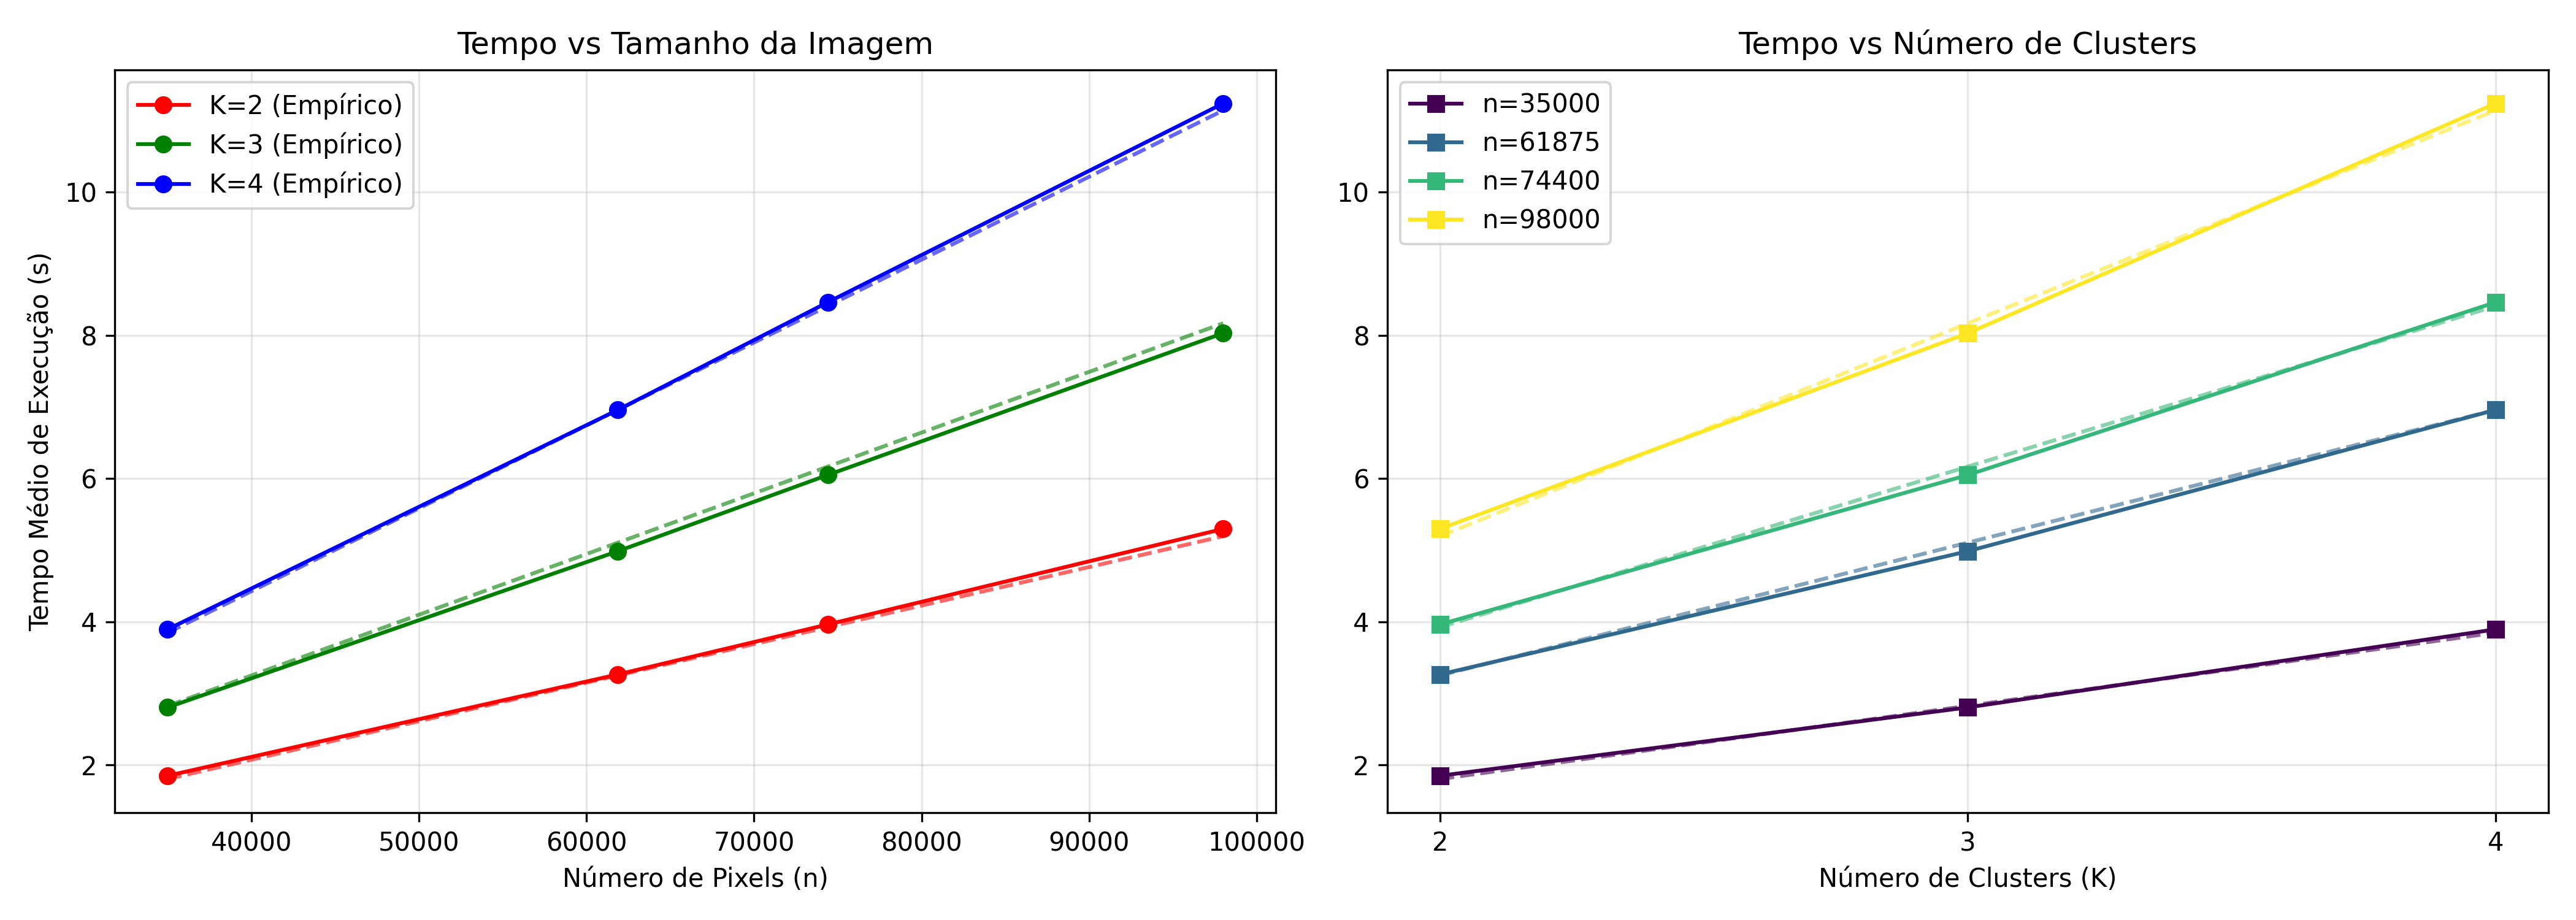
\includegraphics[width=1\textwidth]{relatorio_complexidade.png}
    \caption{Tempo empírico segmentado: $T \times n$ (esquerda) e $T \times K$ (direita). Linhas cheias: médias medidas; tracejadas: modelo ajustado.}
    \label{fig:2d}
\end{figure}

\begin{figure}[h!]
    \centering
    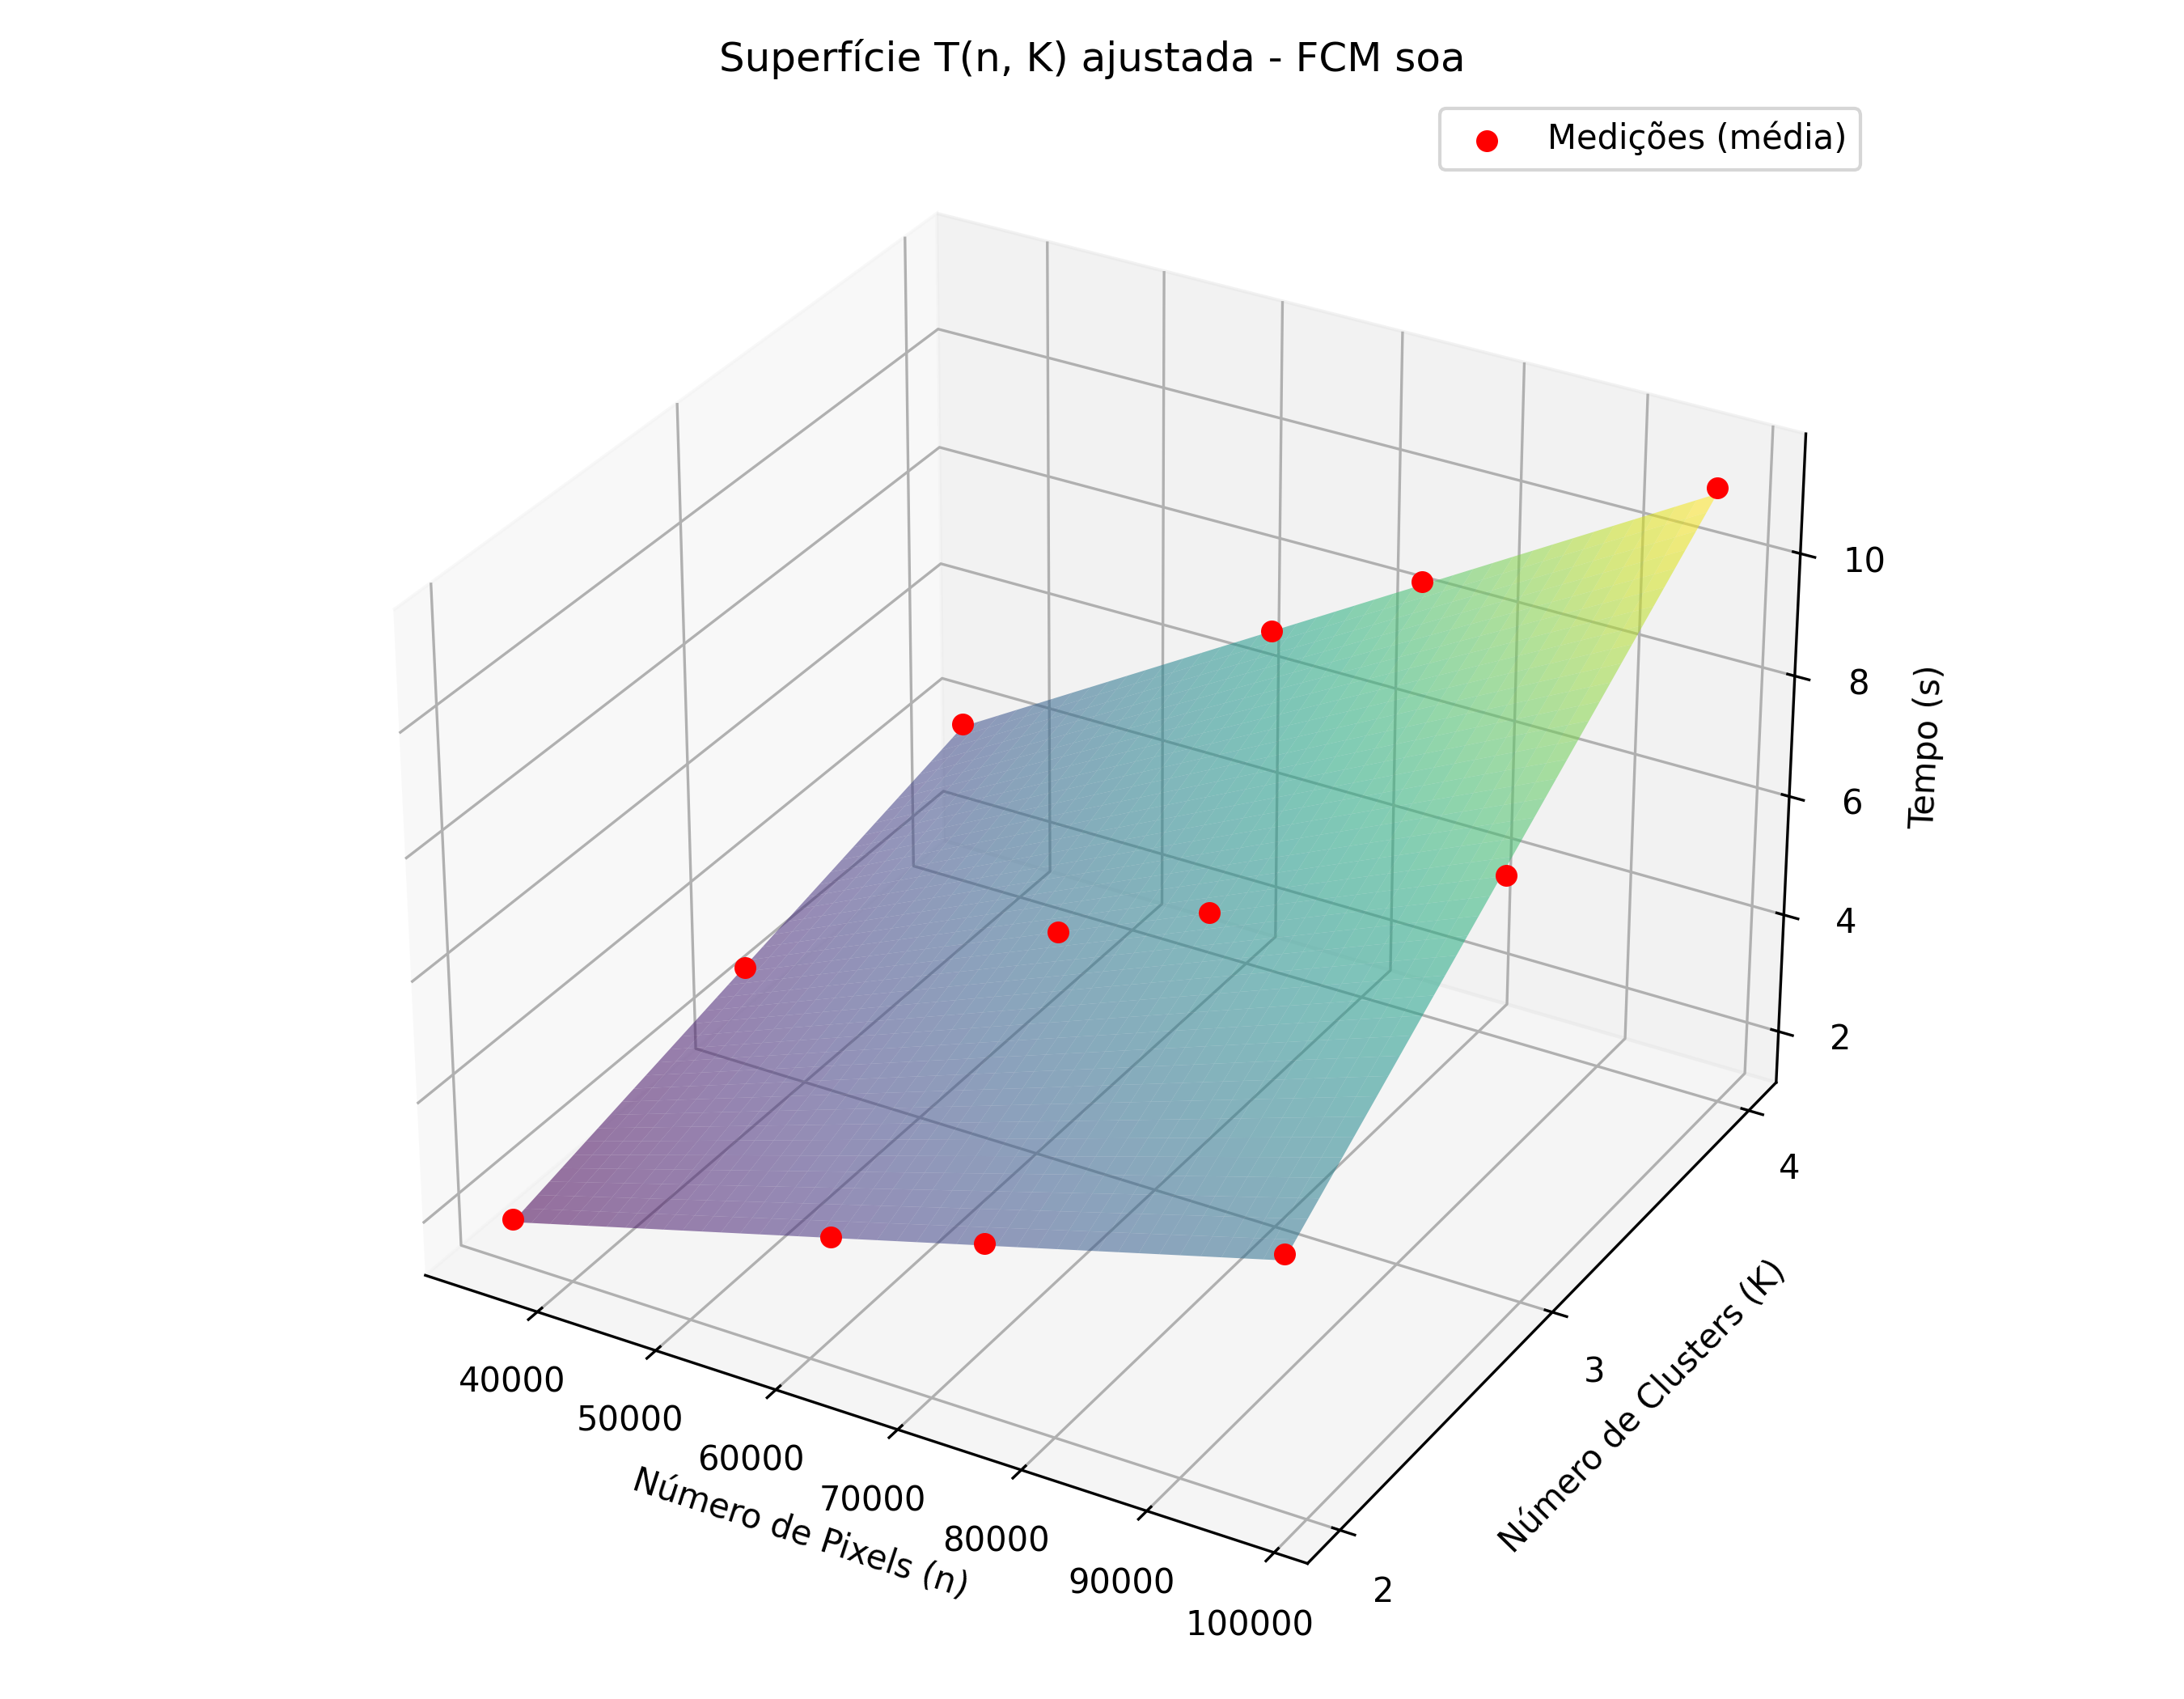
\includegraphics[width=0.8\textwidth]{superficie_3d_foca.png}
    \caption{Superfície de Tempo 3D sobreposta aos pontos de calibração empírica.}
    \label{fig:3d}
\end{figure}

\subsection{Sinal negativo de $\beta$ e $\gamma$}
Os coeficientes $\beta$ e $\gamma$ saíram negativos, o que não tem significado físico (um pixel ou um cluster a mais não pode reduzir o tempo). Isso não indica erro de medição: o modelo da disciplina não tem um termo que existe no algoritmo. No cálculo da pertinência (Fases 3 e 4), o laço \texttt{for k in range(K)} está dentro do laço \texttt{for j in range(K)}, de modo que cada iteração custa da ordem de $nK^2$, e não apenas $nK$. Os tempos medidos mostram isso: para $n = 98000$, o tempo dividido por $K$ cresce de 2,65 s ($K=2$) para 2,68 s ($K=3$) e 2,81 s ($K=4$). Sem o termo $nK^2$, o ajuste compensa a curvatura com $\beta$ e $\gamma$ negativos. Como verificação, ao acrescentar um termo $nK^2$ ao modelo, $\beta$ passa a ser positivo e o $R^2$ sobe para 0,9999. A equação oficial apresentada acima mantém o modelo da disciplina.

\subsection{Comparação com o código Puro (grupo controle)}
\label{sec:comparacao}
O código Puro foi medido na mesma bancada, com os mesmos parâmetros. A Tabela \ref{tab:comparacao} compara os coeficientes das duas variantes.

\begin{table}[h!]
\centering
\caption{Coeficientes de $T_{exp}(n, K)$ para as variantes Puro e SoA}
\label{tab:comparacao}
\begin{tabular}{@{}lccccc@{}}
\toprule
\textbf{Variante} & $\alpha$ & $\beta$ & $\gamma$ & $\delta$ & $R^2$ \\ \midrule
Puro (AoS) & $3{,}1448 \cdot 10^{-5}$ & $-6{,}9811 \cdot 10^{-6}$ & $-5{,}1184 \cdot 10^{-2}$ & $1{,}7239 \cdot 10^{-2}$ & 0,9989 \\
SoA & $3{,}0978 \cdot 10^{-5}$ & $-8{,}1354 \cdot 10^{-6}$ & $-6{,}2831 \cdot 10^{-2}$ & $4{,}6328 \cdot 10^{-2}$ & 0,9991 \\ \bottomrule
\end{tabular}
\end{table}

A variante SoA foi \textbf{mais rápida} que a Puro em todas as 12 combinações, entre 2,7\% e 4,5\% (3,2\% em média), e seu $\alpha$ é 1,5\% menor. O resultado contraria a previsão da missão de que a SoA seria mais lenta por perda de localidade de cache, e é coerente com a análise da Seção 2: no CPython, as listas guardam ponteiros para objetos \texttt{float} espalhados no \textit{heap}, então o layout AoS não oferecia localidade a ser perdida. A explicação mais provável para o pequeno ganho é que a SoA não cria um objeto lista para cada pixel, embora esse efeito não tenha sido medido isoladamente. Como as duas variantes foram medidas uma após a outra, parte da diferença pode vir de variações da máquina entre as rodadas; a consistência do sinal nas 12 combinações, porém, indica que o efeito é real.

\section{Conclusão Parcial}
Os dados atestam que, na faixa medida ($K \le 4$), o tempo da implementação SoA do FCM é descrito pelo modelo de ordem $\mathcal{O}(nK)$ com $R^2 = 0{,}9991$, com o custo concentrado no coeficiente dominante $\alpha$. A análise dos coeficientes revela, porém, um termo $nK^2$ no cálculo da pertinência, que deverá aparecer explicitamente na contagem analítica.

Quanto à restrição arquitetural, a separação estrutural dos canais não produziu a penalidade de cache prevista: no CPython, a variante SoA foi cerca de 3\% mais rápida que o código Puro, porque o interpretador já armazena cada valor como um objeto independente no \textit{heap}. O gargalo de localidade espacial descrito pela missão é uma propriedade de layouts contíguos de memória, e não se manifesta com listas Python.

Este modelo empírico servirá como base absoluta (\textit{ground truth}) para o confronto teórico exigido no Crédito 3 utilizando a contagem F.O.C.A., que deverá incluir o termo $nK^2$ e a diferença de atribuições na montagem da imagem.

\end{document}
